% Options for packages loaded elsewhere
\PassOptionsToPackage{unicode}{hyperref}
\PassOptionsToPackage{hyphens}{url}
%
\documentclass[
]{article}
\usepackage{lmodern}
\usepackage{amssymb,amsmath}
\usepackage{ifxetex,ifluatex}
\ifnum 0\ifxetex 1\fi\ifluatex 1\fi=0 % if pdftex
  \usepackage[T1]{fontenc}
  \usepackage[utf8]{inputenc}
  \usepackage{textcomp} % provide euro and other symbols
\else % if luatex or xetex
  \usepackage{unicode-math}
  \defaultfontfeatures{Scale=MatchLowercase}
  \defaultfontfeatures[\rmfamily]{Ligatures=TeX,Scale=1}
\fi
% Use upquote if available, for straight quotes in verbatim environments
\IfFileExists{upquote.sty}{\usepackage{upquote}}{}
\IfFileExists{microtype.sty}{% use microtype if available
  \usepackage[]{microtype}
  \UseMicrotypeSet[protrusion]{basicmath} % disable protrusion for tt fonts
}{}
\makeatletter
\@ifundefined{KOMAClassName}{% if non-KOMA class
  \IfFileExists{parskip.sty}{%
    \usepackage{parskip}
  }{% else
    \setlength{\parindent}{0pt}
    \setlength{\parskip}{6pt plus 2pt minus 1pt}}
}{% if KOMA class
  \KOMAoptions{parskip=half}}
\makeatother
\usepackage{xcolor}
\IfFileExists{xurl.sty}{\usepackage{xurl}}{} % add URL line breaks if available
\IfFileExists{bookmark.sty}{\usepackage{bookmark}}{\usepackage{hyperref}}
\hypersetup{
  pdftitle={Drug sensitivity in cancer cell lines},
  pdfauthor={DAntoni, Marquard, Neumann, Zymela},
  hidelinks,
  pdfcreator={LaTeX via pandoc}}
\urlstyle{same} % disable monospaced font for URLs
\usepackage[margin=1in]{geometry}
\usepackage{graphicx,grffile}
\makeatletter
\def\maxwidth{\ifdim\Gin@nat@width>\linewidth\linewidth\else\Gin@nat@width\fi}
\def\maxheight{\ifdim\Gin@nat@height>\textheight\textheight\else\Gin@nat@height\fi}
\makeatother
% Scale images if necessary, so that they will not overflow the page
% margins by default, and it is still possible to overwrite the defaults
% using explicit options in \includegraphics[width, height, ...]{}
\setkeys{Gin}{width=\maxwidth,height=\maxheight,keepaspectratio}
% Set default figure placement to htbp
\makeatletter
\def\fps@figure{htbp}
\makeatother
\setlength{\emergencystretch}{3em} % prevent overfull lines
\providecommand{\tightlist}{%
  \setlength{\itemsep}{0pt}\setlength{\parskip}{0pt}}
\setcounter{secnumdepth}{-\maxdimen} % remove section numbering

\title{Drug sensitivity in cancer cell lines}
\author{DAntoni, Marquard, Neumann, Zymela}
\date{19 7 2021}

\begin{document}
\maketitle

\begin{verbatim}
## Warning: package 'dplyr' was built under R version 4.0.5
\end{verbatim}

\begin{verbatim}
## 
## Attaching package: 'dplyr'
\end{verbatim}

\begin{verbatim}
## The following objects are masked from 'package:stats':
## 
##     filter, lag
\end{verbatim}

\begin{verbatim}
## The following objects are masked from 'package:base':
## 
##     intersect, setdiff, setequal, union
\end{verbatim}

\begin{verbatim}
## Warning: package 'svDialogs' was built under R version 4.0.5
\end{verbatim}

\hypertarget{introduction}{%
\section{Introduction:}\label{introduction}}

Developing new drugs against certain diseases always is combined with
high costs, hard work and complicated requirements before even reaching
the market. Therefore an alternative approach of repurposing already
approved drugs to new diseases displays an attractive method to save
time and resources. On top of that by researching further with these
already licensed drugs most safety concerns can be eliminated, since the
medications have been thoroughly tested in previous investigations. All
in all the potential that drug repurposing possesses helps researchers
to create new therapy approaches without the excessive use of follow-up
investigations (Pushpakom et al., 2019).

In our research, we worked with multiple datasets that display among
other things the growth-inhibitory activity of 4518 different drugs
against 481 human cancer cell lines. Here we directed our attention
towards pancreatic cancer cell lines, of which there were 33 found in
the data provided (Corsello et al., 2020).

The most important datasets we focused on in our research were:\\
- the prism Dataset -\textgreater{} containing the treatment effects of
the different cell lines\\
- the prism.exp Dataset -\textgreater{} containing the gene expression
levels for every cell line gene\\
- the prism.achilles -\textgreater{} containing the gene knockdown score
for all cell line genes

The following questions we tried to answer over the course of our
research:\\
- can we identify certain genes that are related to pancreatic cell
lines\\
- can we determine treatments against these pancreatic cell line genes

\hypertarget{data-clean-up}{%
\section{Data Clean-up:}\label{data-clean-up}}

The first step in our research was to clean up the Datasets. This meant
to get rid of all N/A values that would interfere with our findings. The
prism.exp dataset did not contain any of these missing values, hence no
further clean up steps were necessary. The prism and the prism.achilles
dataset on the other hand did possess some N/A values. Here we
{[}\ldots\ldots\ldots.{]}

\hypertarget{descriptive-statistics}{%
\section{Descriptive Statistics:}\label{descriptive-statistics}}

Afterwards we tried to visualize the given datasets to obtain a greater
knowledge about their distribution using different dicriptive
statistical methods.

\hypertarget{prism-dataset}{%
\subsection{prism dataset}\label{prism-dataset}}

Here we tried to display the data containing the different treatment
effects for each cell lines via a heatmap.

\hypertarget{prism.exp-dataset-cell-lines}{%
\subsection{prism.exp dataset cell
lines}\label{prism.exp-dataset-cell-lines}}

For this dataset we checked the distribution of the mean gene values of
all 481 human cancer cell lines to observe some initial characteristics.
This was done using a simple histogram.
\includegraphics{Drug-sensitivity-in-cancer-cell-lines_files/figure-latex/unnamed-chunk-1-1.pdf}

\hypertarget{using-a-statistical-test-to-greatly-reduce-the-number-of-genes-of-interest}{%
\section{Using a statistical test to greatly reduce the number of genes
of
interest}\label{using-a-statistical-test-to-greatly-reduce-the-number-of-genes-of-interest}}

After basic data cleanup and evaluation of the data set prism.exp, which
contained expression data of the cell lines on genes, we were looking
for meaningful criteria with which to reduce the data set. It was clear
that our group should initially focus on the pancreatic cancer cell
lines. A reduction by pancreatic cell lines diminished the expression
data set from 477 to 33 rows. To achieve this, we first used the
metadata set prism.cl to get Depmap IDs, which are assigned to
pancreatic cancer. Since the row names of the prism.exp data set
received the Depmap ID's, we could cut the data set down.

In contrast, identifying interesting genes that are relevant to us
turned out to be more difficult. First, it had to be clear what exactly
was being searched for. Above all, the aim was to find genes that had
distinctive expressions. Such genes whose expression differed
significantly from other cancer cell lines. For such a task there are
competent methods in statistics, which were also discussed in our
bioinformatics lecture. With the help of statistical tests, it is
possible to test hypotheses between values of two cohorts and to
calculate a p-value, which represents a probability with which a
hypothesis can be rejected. For this reason, a corresponding H0
hypothesis was set up for the expression data, paying particular
attention to the mean values.

H0: ``The mean expression of gene X between pancreatic cancer cell lines
and non-pancreatic cancer cell lines is equal''\\
H1: ``The mean expression of gene X between pancreatic cancer cell lines
and non-pancreatic cancer cell lines is different''

One gene from the cohort of 33 pancreatic cancer cell lines and a cohort
of 33 randomly selected other cancer cell lines were examined for
significant deviations from the mean. Since we were using non-normalized
values, we had to use a non-parametric test. Furthermore, we are going
to use two-samples, which are unpaired. For that reason, we were using
the Wilcoxon Rank Sum Test. In this process, the values of the two
groups are combined and given a rank, whereby the information on group
membership is not lost. A test statistic is calculated from this, which
takes the sum of the ranks in a group into account. The result of the
test statistic is compared with critical values, the smaller the result,
the more significant the H0 hypothesis can be rejected.

First, in addition to the data frame, which contained cell lines and
genes, a data frame with the same number of genes in the same order but
with 33 other randomly selected cancer cell lines had to be made. A
prism.exp data frame was created for this, which did not contain any
pancreatic cancer cell lines. 33 cell lines were randomly selected from
this new data frame using the sample function. So, we got two cohorts.

33 values of a gene in one group were compared with 33 values of the
same gene in the other pancreatic cancer-free group using the Wilcoxon
rank sum test. That alone was not enough to find interesting genes. We
had to do the same with all 19177 genes in the data frame. So, a
multiple hypothesis test. For this reason, a for loop was used, which
took over the procedure column by column. For each gene, the calculated
p-value was put into a variable, so that in the end a variable with
19177 values was obtained. Now we can convert the p-values into Boolean
values, according to whether these values reach a given significance
level alpha or not. It must be noted that the significance level must be
adjusted in the case of multiple hypothesis tests, as otherwise the
results will be greatly changed by false positive values at high
implementation rates. We simply used the Bonferroni correction, whereby
the significance value alpha is divided by the number of times, in this
case 19177. Any NA values have been replaced by FALSE. This made it
possible to produce a vector that contained the names that were
significant. The colnames vector of one of the cohorts that had the same
sequence of gene names was used for that.

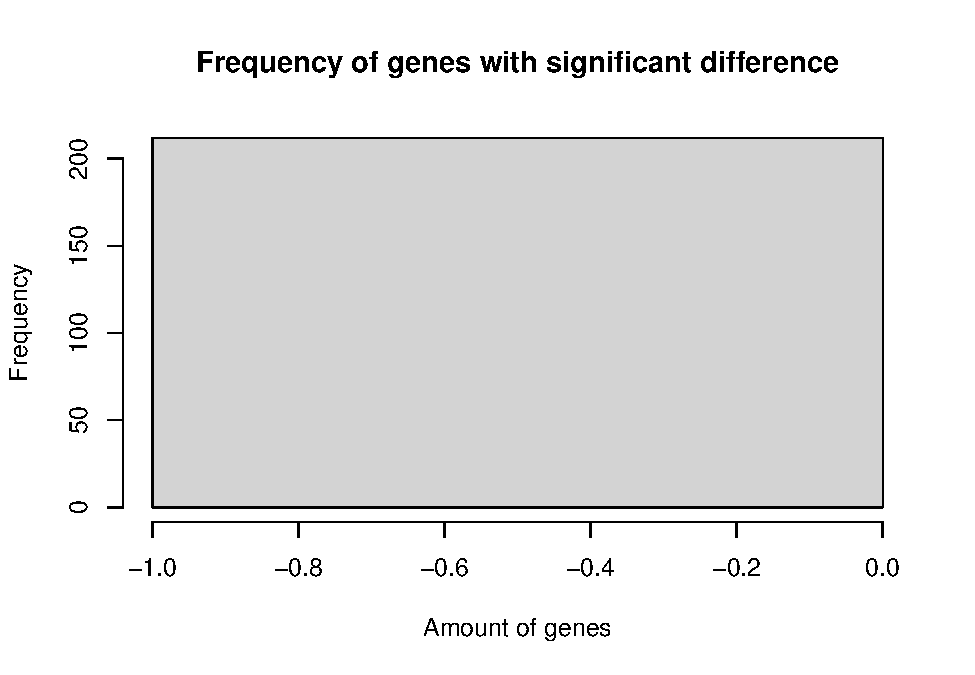
\includegraphics{Drug-sensitivity-in-cancer-cell-lines_files/figure-latex/unnamed-chunk-4-1.pdf}
We can see in this distribution that there is a small group of genes
that regularly differs in the wilcoxon test. Therefore we can reject our
previously established H0 hypothesis.

\begin{verbatim}
##   interesting.genes Freq
## 1              ABL2    1
## 2            ACTR1B    1
## 3             ALPK1    1
## 4          AMMECR1L    1
## 5           ANAPC15    1
## 6           ANKRD60    1
\end{verbatim}

The names of the top interesting genes can be viewed in this data frame.
Here for each gene is the number of times the H0 hypothesis was
discarded for this gene after carrying out onehundred.

\hypertarget{treatment-dataset}{%
\section{Treatment dataset}\label{treatment-dataset}}

\hypertarget{setup-and-initiation}{%
\subsection{Setup and Initiation}\label{setup-and-initiation}}

First we removed all variables of the global environment and loaded in
all functions, data, and packages to be used. Furthermore, all data sets
to be used had their information void columns and rows removed. Then all
prism data were dose correlated, meaning that a drugs effect on cell
growth is normalised to the applied dosage (doscor). Morevover, this
doscor data is further processed, where the mean was taken of each
drug's effect per dosage (perdrug). All three---prism, prism.doscor, and
prism.perdrug---are then split each into a data set, containing only
data for pancreatic cancer cell lines and further into data sets, each
containing only cell lines of one of the four subtypes of pancreatic
cancer as identified in prism.treat. Then we identified the most
efficacious drugs in regards to their ability to inhabit cell growth per
applied dosage. To this end we extracted the drugs above the 95th
percentile for each of the six data sets: prism.perdrug, pancan.perdrug,
and the four perdrug data frames for the four subtypes of pancreatic
cancer.

\hypertarget{having-a-look-at-the-most-effective-drugs}{%
\section{Having a look at the most effective
drugs}\label{having-a-look-at-the-most-effective-drugs}}

Here we take a look at most effective 5\% of drugs, together with their
mean effect per dosage.

\begin{verbatim}
## ef.pancan.perdrug
\end{verbatim}

\begin{verbatim}
## $`exatecan-mesylate`
## [1] -747.9651
## 
## $`SB-743921`
## [1] -660.5004
## 
## $triptolide
## [1] -641.4677
\end{verbatim}

Here we can see that exatecan-mesylate is the drug that has the highest
effect per dosage across all dosages.

\hypertarget{preparing-data-for-kmeans-clustering}{%
\section{Preparing data for kmeans
clustering}\label{preparing-data-for-kmeans-clustering}}

To cluster our cell lines in respect to drug efficacies per dosage, we
decided to only use the 100 drugs with the highest variance. To check
how many clusters are reasonable we used the elbow method.

\begin{verbatim}
## Warning in df.NA.to.val(pancan.perdrug, 2, "median"): 'dim(X)[1]' is relatively
## small at dim(X)[1]==33. Please ensure that imputation along the chosen margin 2
## is robust.

## Warning in df.NA.to.val(pancan.perdrug, 2, "median"): 'dim(X)[1]' is relatively
## small at dim(X)[1]==33. Please ensure that imputation along the chosen margin 2
## is robust.
\end{verbatim}

\includegraphics{Drug-sensitivity-in-cancer-cell-lines_files/figure-latex/unnamed-chunk-8-1.pdf}

\hypertarget{k-means-clustering}{%
\section{K-means clustering}\label{k-means-clustering}}

Since the above graph exhibited a kink at i = 2 we chose to use two
clusters.

\begin{verbatim}
##              Length Class  Mode   
## cluster       33    -none- numeric
## centers      200    -none- numeric
## totss          1    -none- numeric
## withinss       2    -none- numeric
## tot.withinss   1    -none- numeric
## betweenss      1    -none- numeric
## size           2    -none- numeric
## iter           1    -none- numeric
## ifault         1    -none- numeric
\end{verbatim}

To further verify, that our choice of two clusters is the best choice,
we check which amount of clusters has the highest average silhouette
width. The result shows us that a clustering with two clusters is
optimal.

\begin{verbatim}
##  [1] 0.15687127 0.09708832 0.05149854 0.05552384 0.05657905 0.05603248
##  [7] 0.05823367 0.05368667 0.05407538 0.05019621 0.05021786 0.05492287
## [13] 0.04600504 0.04957508 0.05231767 0.04572642 0.04446389 0.03936107
## [19] 0.04247993 0.04400559 0.04554871 0.04267169 0.03884490 0.04002622
## [25] 0.04000158 0.03509645 0.02640868 0.02474554 0.01923425 0.01241012
## [31] 0.00413415
\end{verbatim}

\begin{verbatim}
## [1] 0.1568713
\end{verbatim}

\begin{verbatim}
## [1] 2
\end{verbatim}

\includegraphics{Drug-sensitivity-in-cancer-cell-lines_files/figure-latex/unnamed-chunk-10-1.pdf}

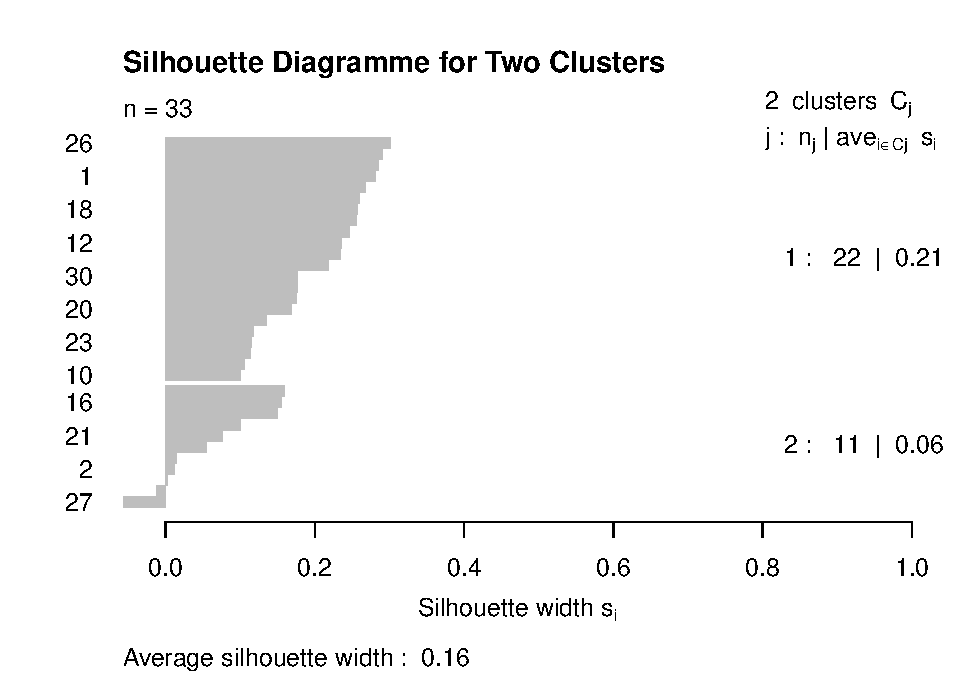
\includegraphics{Drug-sensitivity-in-cancer-cell-lines_files/figure-latex/unnamed-chunk-11-1.pdf}

\hypertarget{regression-analysis}{%
\section{Regression Analysis}\label{regression-analysis}}

\hypertarget{preparation-for-regression-analysis}{%
\subsection{Preparation for Regression
Analysis}\label{preparation-for-regression-analysis}}

We extract all data regarding pancreatic cancer cell lines from the
prism.achilles data set. Then we extract information about the top 2
drugs in regard to their ability to inhibit cell growth. We then define
a fitted pancan.achilles data frame for each of the five drugs, that
contains only the cell lines where we have drug efficacy data and visa
versa.

\begin{verbatim}
##  [1] "dr.ef.pancan.max.1"       "dr.ef.pancan.max.2"      
##  [3] "dr.ef.pancan.max.3"       "dr.ef.pancan.max.4"      
##  [5] "dr.ef.pancan.max.5"       "ef.pancan.max.percl.1"   
##  [7] "ef.pancan.max.percl.2"    "ef.pancan.max.percl.3"   
##  [9] "ef.pancan.max.percl.4"    "ef.pancan.max.percl.5"   
## [11] "id.dr.ef.pancan.max.1"    "id.dr.ef.pancan.max.2"   
## [13] "id.dr.ef.pancan.max.3"    "id.dr.ef.pancan.max.4"   
## [15] "id.dr.ef.pancan.max.5"    "pancan.achilles"         
## [17] "pancan.achilles.fitted.1" "pancan.achilles.fitted.2"
## [19] "pancan.achilles.fitted.3" "pancan.achilles.fitted.4"
## [21] "pancan.achilles.fitted.5"
\end{verbatim}

We now set up our data upon which our linear regression will be based.
We here only use the 5th percentile of the achilles gene data of the
highest variance.

\begin{verbatim}
## Warning in df.NA.to.val(.env.ra[[paste("pancan.achilles.fitted.", j, sep =
## "")]], : 'dim(X)[1]' is relatively small at dim(X)[1]==24. Please ensure that
## imputation along the chosen margin 2 is robust.
\end{verbatim}

\begin{verbatim}
## Warning in df.NA.to.val(.env.ra[[paste("pancan.achilles.fitted.", j, sep =
## "")]], : 'dim(X)[1]' is relatively small at dim(X)[1]==25. Please ensure that
## imputation along the chosen margin 2 is robust.
\end{verbatim}

\hypertarget{regression-analysis-1}{%
\subsection{Regression analysis}\label{regression-analysis-1}}

Now we perform the regression analysis for the two best drugs in regard
to their ability to inhabit cell growth in pancreatic cancer cell lines.

\begin{verbatim}
## [1] 0.3412674
## [1] "MIPEP"
## [1] 432
## [1] 0.5502163
## [1] "FBXO11"
## [1] 259
\end{verbatim}

\includegraphics{Drug-sensitivity-in-cancer-cell-lines_files/figure-latex/unnamed-chunk-15-1.pdf}

\includegraphics{Drug-sensitivity-in-cancer-cell-lines_files/figure-latex/unnamed-chunk-16-1.pdf}

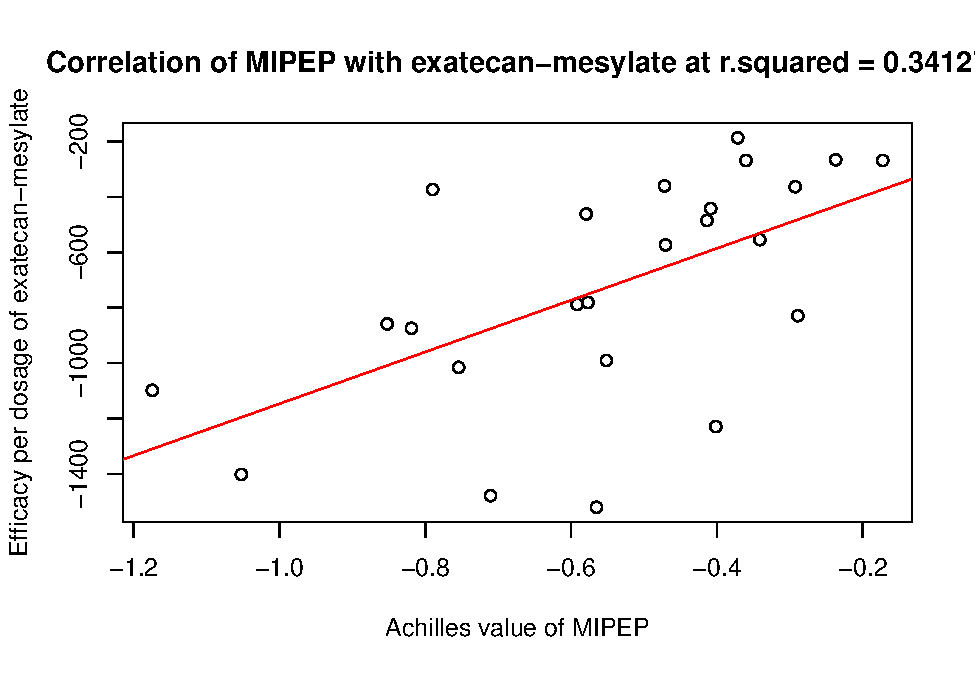
\includegraphics{Drug-sensitivity-in-cancer-cell-lines_files/figure-latex/unnamed-chunk-17-1.pdf}

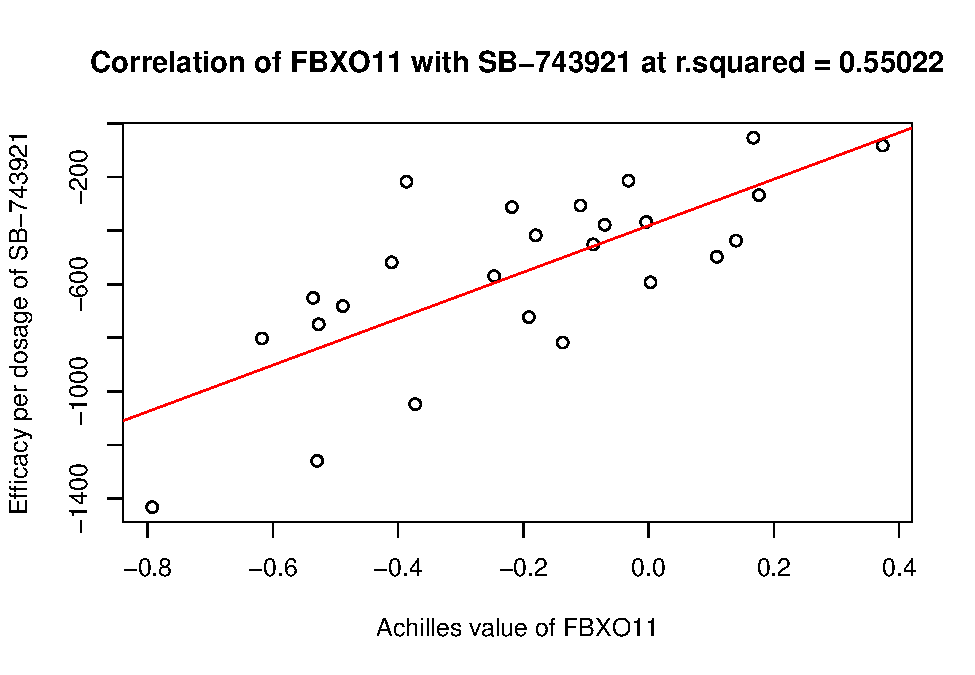
\includegraphics{Drug-sensitivity-in-cancer-cell-lines_files/figure-latex/unnamed-chunk-18-1.pdf}

\begin{verbatim}
## Warning: package 'ggpubr' was built under R version 4.0.5
\end{verbatim}

4 prism.achilles

4.1 Cleanup of prism.achilles

4.1.1 na removal

\begin{verbatim}
## [1] 277 323
\end{verbatim}

\begin{verbatim}
## [1] -0.028821097  0.092031824           NA  0.100156084  0.051651937
## [6] -0.003150406
\end{verbatim}

\begin{verbatim}
## [1] -0.21325586 -0.06681872  0.25195944          NA -0.08459803  0.09666667
\end{verbatim}

\begin{verbatim}
## [1] "ACH-000836" "ACH-000901" "ACH-000939"
\end{verbatim}

\begin{verbatim}
## [1] 3302
\end{verbatim}

\begin{verbatim}
## [1] 0
\end{verbatim}

\begin{verbatim}
## [1]   347 18119
\end{verbatim}

4.1.2 Make Prism.achilles numeric

10.Intermission - Sort Prism.cl by depmap\_id resulting in
prism.cl.ordered

\begin{verbatim}
##             DepMap_ID stripped_cell_line_name            CCLE_Name
## ACH-000052 ACH-000052                    A673            A673_BONE
## ACH-000082 ACH-000082         G292CLONEA141B1 G292CLONEA141B1_BONE
## ACH-000087 ACH-000087                   SKES1           SKES1_BONE
\end{verbatim}

\begin{verbatim}
## [1] 481  41
\end{verbatim}

\begin{verbatim}
##  [1] "1"  "2"  "3"  "4"  "5"  "6"  "7"  "8"  "9"  "10" "11" "12" "13" "14" "15"
## [16] "16" "17" "18" "19" "20" "21" "22" "23" "24" "25" "26" "27" "28" "29" "30"
\end{verbatim}

\begin{verbatim}
##     DepMap_ID stripped_cell_line_name                     CCLE_Name
## 1  ACH-000007                   LS513         LS513_LARGE_INTESTINE
## 2  ACH-000008                   A101D                    A101D_SKIN
## 3  ACH-000011                    253J            253J_URINARY_TRACT
## 4  ACH-000012                  HCC827                   HCC827_LUNG
## 5  ACH-000013                 ONCODG1                 ONCODG1_OVARY
## 6  ACH-000014                  HS294T                   HS294T_SKIN
## 7  ACH-000015                NCIH1581                 NCIH1581_LUNG
## 8  ACH-000018                     T24             T24_URINARY_TRACT
## 9  ACH-000019                    MCF7                   MCF7_BREAST
## 10 ACH-000021                NCIH1693                 NCIH1693_LUNG
## 11 ACH-000022               PATU8988S            PATU8988S_PANCREAS
## 12 ACH-000023               PATU8988T            PATU8988T_PANCREAS
## 13 ACH-000026                  253JBV          253JBV_URINARY_TRACT
## 14 ACH-000027                    GOS3   GOS3_CENTRAL_NERVOUS_SYSTEM
## 15 ACH-000030                    PC14                     PC14_LUNG
## 16 ACH-000035                NCIH1650                 NCIH1650_LUNG
## 17 ACH-000037                    S117                  S117_THYROID
## 18 ACH-000040                  U118MG U118MG_CENTRAL_NERVOUS_SYSTEM
## 19 ACH-000042                PANC0203             PANC0203_PANCREAS
## 20 ACH-000046                    ACHN                   ACHN_KIDNEY
## 21 ACH-000047                    GCIY                  GCIY_STOMACH
## 22 ACH-000048                 TOV112D                 TOV112D_OVARY
## 23 ACH-000052                    A673                     A673_BONE
## 24 ACH-000054                  HT1080            HT1080_SOFT_TISSUE
## 25 ACH-000060                PANC1005             PANC1005_PANCREAS
## 26 ACH-000062                RERFLCMS                 RERFLCMS_LUNG
## 27 ACH-000066                 HCC4006                  HCC4006_LUNG
## 28 ACH-000082         G292CLONEA141B1          G292CLONEA141B1_BONE
## 29 ACH-000086                ACCMESO1               ACCMESO1_PLEURA
## 30 ACH-000087                   SKES1                    SKES1_BONE
\end{verbatim}

\begin{verbatim}
## [1] 347  41
\end{verbatim}

\begin{verbatim}
## [1] "ACH-000007" "ACH-000011" "ACH-000012" "ACH-000013" "ACH-000014"
\end{verbatim}

\begin{verbatim}
## [1] "ACH-000007" "ACH-000011" "ACH-000012" "ACH-000013" "ACH-000014"
\end{verbatim}

Find PanCan Cellines in prism.cl.achilles

\begin{verbatim}
##  [1] "Pancreatic Cancer" "Pancreatic Cancer" "Pancreatic Cancer"
##  [4] "Pancreatic Cancer" "Pancreatic Cancer" "Pancreatic Cancer"
##  [7] "Pancreatic Cancer" "Pancreatic Cancer" "Pancreatic Cancer"
## [10] "Pancreatic Cancer" "Pancreatic Cancer" "Pancreatic Cancer"
## [13] "Pancreatic Cancer" "Pancreatic Cancer" "Pancreatic Cancer"
## [16] "Pancreatic Cancer" "Pancreatic Cancer" "Pancreatic Cancer"
## [19] "Pancreatic Cancer" "Pancreatic Cancer" "Pancreatic Cancer"
## [22] "Pancreatic Cancer" "Pancreatic Cancer" "Pancreatic Cancer"
## [25] "Pancreatic Cancer"
\end{verbatim}

\begin{verbatim}
##  [1] "ACH-000022" "ACH-000042" "ACH-000060" "ACH-000108" "ACH-000118"
##  [6] "ACH-000138" "ACH-000164" "ACH-000178" "ACH-000222" "ACH-000235"
## [11] "ACH-000243" "ACH-000265" "ACH-000266" "ACH-000281" "ACH-000307"
## [16] "ACH-000320" "ACH-000332" "ACH-000468" "ACH-000502" "ACH-000517"
## [21] "ACH-000535" "ACH-000599" "ACH-000601" "ACH-000652" "ACH-000685"
\end{verbatim}

\begin{verbatim}
##  [1] "ACH-000022" "ACH-000042" "ACH-000060" "ACH-000108" "ACH-000118"
##  [6] "ACH-000138" "ACH-000164" "ACH-000178" "ACH-000222" "ACH-000235"
## [11] "ACH-000243" "ACH-000265" "ACH-000266" "ACH-000281" "ACH-000307"
## [16] "ACH-000320" "ACH-000332" "ACH-000468" "ACH-000502" "ACH-000517"
## [21] "ACH-000535" "ACH-000599" "ACH-000601" "ACH-000652" "ACH-000685"
\end{verbatim}

\begin{verbatim}
##  [1] "1"  "2"  "3"  "4"  "5"  "6"  "7"  "8"  "9"  "10"
\end{verbatim}

\begin{verbatim}
##  [1] "ACH-000007" "ACH-000011" "ACH-000012" "ACH-000013" "ACH-000014"
##  [6] "ACH-000015" "ACH-000018" "ACH-000019" "ACH-000021" "ACH-000022"
\end{verbatim}

\begin{verbatim}
##  [1] "ACH-000007" "ACH-000011" "ACH-000012" "ACH-000013" "ACH-000014"
##  [6] "ACH-000015" "ACH-000018" "ACH-000019" "ACH-000021" "ACH-000022"
\end{verbatim}

The data frame prism.achilles consists of gene knockdown scores. The
score is a measure of how essential/important is a particular gene for
the cell survival. This score reflects whether upon knocking down that
genes does the cell reduce its proliferation or increases it or has no
change. Smaller values refers to higher essentiality. The rows of this
matrix are the gene names and the columns are the cancer cell line
identifiers.

Exploration of prism.achilles.numeric

\begin{verbatim}
## [1]   347 18119
\end{verbatim}

\begin{verbatim}
##                    A1BG         A1CF
## ACH-000007  0.066211918  0.073849767
## ACH-000011  0.270231724  0.072104660
## ACH-000012  0.015445134  0.173129613
## ACH-000013  0.062819955  0.038241805
## ACH-000014  0.137092353 -0.054472837
## ACH-000015 -0.068873122 -0.005479247
## ACH-000018 -0.033071218  0.084952865
## ACH-000019  0.156900046 -0.043868154
## ACH-000021 -0.005489147  0.010287761
## ACH-000022  0.022416059  0.120401365
\end{verbatim}

\begin{verbatim}
##  [1]  10  15  20  29  30  35  42  46  57  62  64  72  73  81  87  94 100 144 160
## [20] 166 171 187 188 204 217
\end{verbatim}

\begin{verbatim}
##   ACH-000022   ACH-000042   ACH-000060   ACH-000108   ACH-000118   ACH-000138 
##  0.022416059  0.060227981  0.077120280 -0.074207796  0.093583325 -0.007891226 
##   ACH-000164   ACH-000178   ACH-000222   ACH-000235 
## -0.013418620  0.099319688  0.053796423  0.175114835
\end{verbatim}

\begin{verbatim}
## [1] TRUE
\end{verbatim}

\includegraphics{Drug-sensitivity-in-cancer-cell-lines_files/figure-latex/unnamed-chunk-28-1.pdf}
\includegraphics{Drug-sensitivity-in-cancer-cell-lines_files/figure-latex/unnamed-chunk-28-2.pdf}

\begin{verbatim}
##           0%          10%          20%          30%          40%          50% 
## -3.013158370 -0.581997749 -0.287929545 -0.182443722 -0.113291797 -0.058112943 
##          60%          70%          80%          90%         100% 
## -0.007522533  0.042161024  0.097314728  0.169981701  2.390190374
\end{verbatim}

\begin{verbatim}
##           0%          10%          20%          30%          40%          50% 
## -4.495161219 -0.595177702 -0.301276609 -0.191269511 -0.118877789 -0.060704660 
##          60%          70%          80%          90%         100% 
## -0.007980654  0.044477885  0.102514805  0.179948353  4.874965251
\end{verbatim}

\begin{verbatim}
##        10% 
## -0.5951777
\end{verbatim}

\begin{verbatim}
##                 A1BG        A1CF         A2M      A2ML1     A3GALT2
## ACH-001239 0.1437121  0.03772355 -0.14169312 0.20126637 -0.02146561
## ACH-001306 0.1699559  0.11702571 -0.16983882 0.07760954  0.02798856
## ACH-001318 0.2043360 -0.29032415  0.01755972 0.07387247 -0.10890666
\end{verbatim}

\begin{verbatim}
## [1]   347 18119
\end{verbatim}

\begin{verbatim}
## [1]   347 18119
\end{verbatim}

New Dataframe for Analysis of prism.achilles.numeric

\begin{verbatim}
## [1]  0.43862658  0.08860929 -0.23506619 -0.06972403  0.06241759  0.00000000
## [7]  0.01372463
\end{verbatim}

\begin{verbatim}
## [1]  4283  7638  7955 17229
\end{verbatim}

\begin{verbatim}
##                   DOCK5      KCNK13        KRAS         WLS
## max          0.43776386  0.53068373  0.06927002  0.41504652
## mean        -0.08222936 -0.03646742 -0.58201216  0.12194959
## min         -1.26474680 -2.36986289 -2.15523077 -0.80051723
## 10%quantile -0.35935966 -0.14240574 -1.28502818 -0.01467511
## Pancanmean  -0.41593873 -0.44466120 -1.30698799 -0.02380382
## is(r5<r4)    1.00000000  1.00000000  1.00000000  1.00000000
## stdev        0.05767614  0.09384127  0.17246569  0.01692432
\end{verbatim}

\begin{verbatim}
## 
##  Shapiro-Wilk normality test
## 
## data:  prism.achilles.numeric[, 4283]
## W = 0.88736, p-value = 2.696e-15
\end{verbatim}

\begin{verbatim}
## 
##  Shapiro-Wilk normality test
## 
## data:  prism.achilles.numeric[, 7638]
## W = 0.63224, p-value < 2.2e-16
\end{verbatim}

\begin{verbatim}
## 
##  Shapiro-Wilk normality test
## 
## data:  prism.achilles.numeric[, 7955]
## W = 0.84554, p-value < 2.2e-16
\end{verbatim}

\begin{verbatim}
## 
##  Shapiro-Wilk normality test
## 
## data:  prism.achilles.numeric[, 17229]
## W = 0.85977, p-value < 2.2e-16
\end{verbatim}

ggqqplot(prism.achilles.numeric{[},4283{]})
ggqqplot(prism.achilles.numeric{[},7638{]})
ggqqplot(prism.achilles.numeric{[},7955{]})
ggqqplot(prism.achilles.numeric{[},17229{]})

merlinsvariable \textless- 10000 cor.mat.achilles \textless-
cor(prism.achilles.numeric.pancan{[},1:merlinsvariable{]})
cor.mat.achilles{[}779,782{]} interesting.cor.values \textless-
which(cor.mat.achilles \textgreater{} 0.90 \& cor.mat.achilles
\textless{} 1 ) interesting.cor.rows \textless-
(((interesting.cor.values - (interesting.cor.values \%\%
merlinsvariable)) /merlinsvariable) +1) interesting.cor.cols \textless-
(interesting.cor.values \%\% merlinsvariable)
cor.mat.achilles{[}interesting.cor.rows, interesting.cor.cols{]}

k-means clustering

Using the most variable, thus informative genes We first reduce our
dataset to take the most variable gene, which are expected to carry most
of the information about the samples:

\begin{verbatim}
##     Min.  1st Qu.   Median     Mean  3rd Qu.     Max. 
## 0.004248 0.012590 0.015523 0.020433 0.020707 0.503658
\end{verbatim}

\begin{verbatim}
## [1]  347 4530
\end{verbatim}

Clustering by depmap

\begin{verbatim}
## [1] 61682.45
\end{verbatim}

\begin{verbatim}
##   [1] 61682.45 60064.82 59135.66 58227.20 57458.90 56969.90 56495.06 56000.88
##   [9] 55217.80 54763.08 54392.95 54009.66 53510.01 53414.19 52913.11 52410.57
##  [17] 52083.83 51725.04 51409.13 51192.57 50802.95 50531.85 50231.25 49913.30
##  [25] 49561.03 49240.69 48968.93 48622.60 48440.03 47915.00 47767.59 47682.05
##  [33] 47471.40 47107.79 46755.93 46409.11 46314.16 46099.61 45642.89 45406.98
##  [41] 45145.06 44938.57 44747.31 44387.56 44113.80 43812.26 43647.76 43390.85
##  [49] 43096.58 42970.40 42519.76 42531.66 42386.73 41997.45 41836.64 41426.39
##  [57] 41265.85 41092.64 40963.11 40758.40 40438.22 40082.22 39926.13 39743.91
##  [65] 39524.63 39223.94 39066.21 38877.65 38625.13 38373.23 38236.06 38059.72
##  [73] 37827.77 37702.28 37432.55 37342.85 37107.30 36857.47 36741.18 36528.03
##  [81] 36222.31 36136.12 35801.99 35662.33 35499.77 35240.91 34945.26 34855.97
##  [89] 34711.31 34502.20 34305.70 34026.86 33937.00 33803.81 33613.08 33345.27
##  [97] 33147.60 32898.60 32875.20 32573.73
\end{verbatim}

\includegraphics{Drug-sensitivity-in-cancer-cell-lines_files/figure-latex/unnamed-chunk-36-1.pdf}
\includegraphics{Drug-sensitivity-in-cancer-cell-lines_files/figure-latex/unnamed-chunk-36-2.pdf}

\begin{verbatim}
## ACH-000007 ACH-000011 ACH-000012 ACH-000013 ACH-000014 ACH-000015 ACH-000018 
##          1          2          1          1          2          1          2 
## ACH-000019 ACH-000021 ACH-000022 
##          1          1          1
\end{verbatim}

\begin{verbatim}
##              Length Class  Mode   
## cluster       347   -none- numeric
## centers      9060   -none- numeric
## totss           1   -none- numeric
## withinss        2   -none- numeric
## tot.withinss    1   -none- numeric
## betweenss       1   -none- numeric
## size            2   -none- numeric
## iter            1   -none- numeric
## ifault          1   -none- numeric
\end{verbatim}

\begin{verbatim}
##  [1] "ACH-000022" "ACH-000042" "ACH-000060" "ACH-000108" "ACH-000118"
##  [6] "ACH-000138" "ACH-000164" "ACH-000178" "ACH-000222" "ACH-000235"
## [11] "ACH-000243" "ACH-000265" "ACH-000266" "ACH-000281" "ACH-000307"
## [16] "ACH-000320" "ACH-000332" "ACH-000468" "ACH-000502" "ACH-000517"
## [21] "ACH-000535" "ACH-000599" "ACH-000601" "ACH-000652" "ACH-000685"
\end{verbatim}

\begin{verbatim}
## ACH-000022 ACH-000042 ACH-000060 ACH-000108 ACH-000118 ACH-000138 ACH-000164 
##          1          2          2          2          1          1          2 
## ACH-000178 ACH-000222 ACH-000235 ACH-000243 ACH-000265 ACH-000266 ACH-000281 
##          2          2          2          2          1          2          2 
## ACH-000307 ACH-000320 ACH-000332 ACH-000468 ACH-000502 ACH-000517 ACH-000535 
##          1          1          2          2          2          2          1 
## ACH-000599 ACH-000601 ACH-000652 ACH-000685 
##          2          2          1          1
\end{verbatim}

Clustering by genes

\begin{verbatim}
## [1]  347 4530
\end{verbatim}

wss.genes dim(wss.genes) plot(wss.genes{[}100:1000{]}, type=``b'',
xlab=``Number of Clusters'', ylab=``Within groups sum of squares'')
plot(wss.genes{[}100:500{]}, type=``b'', xlab=``Number of Clusters'',
ylab=``Within groups sum of squares'')

\begin{verbatim}
## ACH-000007 ACH-000011 ACH-000012 ACH-000013 ACH-000014 ACH-000015 ACH-000018 
##          2          1          2          2          1          2          1 
## ACH-000019 ACH-000021 ACH-000022 
##          2          2          2
\end{verbatim}

\begin{verbatim}
##              Length Class  Mode   
## cluster       347   -none- numeric
## centers      9060   -none- numeric
## totss           1   -none- numeric
## withinss        2   -none- numeric
## tot.withinss    1   -none- numeric
## betweenss       1   -none- numeric
## size            2   -none- numeric
## iter            1   -none- numeric
## ifault          1   -none- numeric
\end{verbatim}

\begin{verbatim}
##  [1] "ACH-000022" "ACH-000042" "ACH-000060" "ACH-000108" "ACH-000118"
##  [6] "ACH-000138" "ACH-000164" "ACH-000178" "ACH-000222" "ACH-000235"
## [11] "ACH-000243" "ACH-000265" "ACH-000266" "ACH-000281" "ACH-000307"
## [16] "ACH-000320" "ACH-000332" "ACH-000468" "ACH-000502" "ACH-000517"
## [21] "ACH-000535" "ACH-000599" "ACH-000601" "ACH-000652" "ACH-000685"
\end{verbatim}

\begin{verbatim}
## ACH-000022 ACH-000042 ACH-000060 ACH-000108 ACH-000118 ACH-000138 ACH-000164 
##          2          1          1          1          2          2          1 
## ACH-000178 ACH-000222 ACH-000235 ACH-000243 ACH-000265 ACH-000266 ACH-000281 
##          1          1          1          1          2          1          1 
## ACH-000307 ACH-000320 ACH-000332 ACH-000468 ACH-000502 ACH-000517 ACH-000535 
##          2          2          1          1          1          1          2 
## ACH-000599 ACH-000601 ACH-000652 ACH-000685 
##          1          1          2          2
\end{verbatim}

\end{document}
